%!TEX root = ../summaries.tex

\chapter{Learning from humans}

\section{Imitation Learning, Part 1}

\url{https://youtu.be/kGc8jOy5_zY}

\begin{itemize}
    \item Differences when moving from prediction to control for AI systems
    \begin{itemize}
        \item No longer i.i.d.
        \item From ground truth supervision to high-level, abstract goal.
        \item Objective: from predict label to accomplish task.
        \item In real world, some prediction systems also have feedback issues: e.g.\@ traffic prediction system used and affects traffic.
    \end{itemize}
    \item Terminology.
    \begin{itemize}
        \item $\bf o_t$: observation.
        \item $\bf a_t$: action.
        \item $\bf s_t$: state (underlying variables in model).
        \item $\pi_\theta(\bf a_t \mid \bf o_t)$ or $\pi_\theta(\bf a_t \mid \bf s_t)$: policy.
        \item When policy depends on state, it is \emph{fully observed}.
        \begin{figure}[h!]
            \centering
            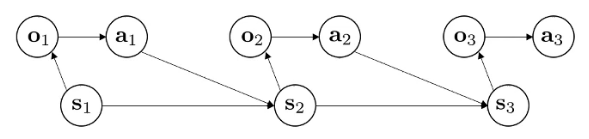
\includegraphics[width=.95\linewidth]{images/state-bayes-net.png}
            \caption{Bayes' net for the states, observations and actions}
            \label{fig:bayes net states}
        \end{figure}
    \end{itemize}
    \item Initiation learning: supervised learning.
    \begin{itemize}
        \item \emph{Behaviour cloning}.
        \item Doesn't work in theory: small mistakes compound, and we quickly diverge from training distribution.
        \item Works reasonably well in practice, given enough training data.
    \end{itemize}
\end{itemize}


\section{Learning from Human Preferences}

\url{https://openai.com/blog/deep-reinforcement-learning-from-human-preferences/}

\begin{itemize}
    \item Using feedback to infer goal.
    \item Builds model of goal based on feedback.
    \item Learns also when to ask for feedback.
    \item Trained on various games.
    \item Sometimes does better using human feedback than game's actual reward function (the score), since human shapes the reward function better.
    \item Limited by human evaluators intuition on what looks correct.
    \begin{itemize}
        \item On one task, learned to trick human using optical illusion.
    \end{itemize}
\end{itemize}


\section{Learning to Summarize with Human Feedback}

\url{https://openai.com/blog/learning-to-summarize-with-human-feedback/}

\begin{itemize}
    \item Used human feedback to train summarisers.
    \item Produced better performance than much larger models trained only with supervised learning.
    \item Models usually trained with objective to predict next word, but what we really want is high-quality summaries.
    \begin{itemize}
        \item Models can make up things when unsure.
        \item Models can imitate harmful social biases.
    \end{itemize}
    \item First train reward model using supervised learning, then fine-tune language model with reinforcement learning.
    \item Provided frequent feedback to human labellers, to ensure that the labellers were marking according to their goals.
    \item Tested generalisation capacity by using a different dataset, with different types of text.
    \begin{itemize}
        \item Model had been pre-trained on these, but had no human feedback.
        \item Produced high-quality summaries.
        \item When length adjusted, produced even better summaries than the human-made samples.
    \end{itemize}
    \item Core method.
    \begin{enumerate}[label=\arabic*.]
        \item Train initial summariser.
        \item Build dataset of human comparisons between summaries.
        \item Train reward model to predict human preference.
        \item Fine-tune summariser using RL and reward model.
    \end{enumerate}
    \item Took care to ensure high-quality human data.
    \item Optimising reward model eventually lead to quality degradation.
    \begin{itemize}
        \item Reward model only a proxy for human preferences.
        \item Trained on relatively small set of summaries.
        \item When the model optimised to the reward too much, it overfit, and produced poor summaries.
    \end{itemize}
    \item Limitations.
    \begin{itemize}
        \item For more complex tasks, unlikely that researcher labels should be taken as `gold standard'.
        \begin{itemize}
            \item Should hire labellers from impacted groups to define `good' behaviour and reinforce it.
        \end{itemize}
        \item Model trained on Reddit data, and sometimes produced harmful summaries.
        \item Used significant compute resources.
        \item Though outperform human reference summaries, those themselves are not rated very highly on axes of quality (accuracy, coverage, coherence, and overall).
    \end{itemize}
\end{itemize}


\section{Inverse Reinforcement Learning Example}

\url{https://www.youtube.com/watch?v=h7uGyBcIeII}

\begin{itemize}
    \item Inferring reward function based on what actions are taken and what actions are not taken.
    \item Maximum likelihood inverse reinforcement learning. Repeat:
    \begin{enumerate}[label=(\roman*)]
        \item Guess reward $R$.
        \item Compute optimal policy $\pi$ for $R$.
        \item Measure $p(D \mid \pi)$.
        \item Gradient on $R$.
    \end{enumerate}
    \item What to do about final states?
    \begin{itemize}
        \item Want to indicate that these are good places to be, so should be there for a while.
        \item But if there too long, it outweigh other actions taken.
    \end{itemize}
\end{itemize}


\section{Learning from humans: what is inverse reinforcement learning?}

\url{https://thegradient.pub/learning-from-humans-what-is-inverse-reinforcement-learning/}

\begin{itemize}
    \item {[}Not so well written. Best to also consult \cite{ng2000algorithms}.]
    \item Generally, algorithms solving IRL can be seen as a way to use expert knowledge to convert a task description into a reward function.
    \item Problem: a policy may be maximal for many different reward functions.
    \item Solution: additionally require that certain properties are maximised (Ng and Russell).
    \begin{itemize}
        \item Maximise difference between quality of optimal solution and next-best, subject to some bound.
        \begin{itemize}
            \item Gives a reward function for which the policy is clearly distinguished.
        \end{itemize}
        \item Minimise reward vector.
        \begin{itemize}
            \item Encourages reward function to be simpler.
            \item Ng and Russell use L1 norm.
        \end{itemize}
    \end{itemize}
    \item Value of policy $\pi$ given reward $R$ and discount factor $\gamma$:
    \begin{equation*}
        V^\pi(s_1) = \bb E[R(s_1) + \gamma R(s_2) + \gamma^2 R(s_3) + \cdots \mid \pi]
    \end{equation*}
    where we take the expectation over the distribution of states $(s_1, s_2, \ldots)$ passed through under the policy.
    \item Using sampled trajectories.
    \begin{itemize}
        \item In most real-world situations, we don't have access to the full policy, but instead to a number of (Monte Carlo) trajectories through it: episodes of applying this policy.
        \item Parametrise reward as:
        \begin{equation*}
            R(s) = \alpha_1 \phi_1(s) +  \cdots + \alpha_d \phi_d(s)
        \end{equation*}
        where $\phi_1, \ldots, \phi_d$ are basis functions chosen beforehand.
        \item We learn the weights $\alpha_1, \ldots, \alpha_d$ from the data (trajectories observed).
        \item Let $\pi^*$ be the hypothetical optimal policy given by human experts.
        \item Sample trajectories from $\pi^*$ and use these to estimate the value of each basis function under this policy.
        \item We can then estimate the value of the full reward, given values $\alpha_1, \ldots, \alpha_d$.
        \item We will do the same for various other policies $\pi_1, \pi_2, \ldots$.
        \item The way the algorithm works:
        \begin{itemize}
            \item Start with a random policy $\pi_1$.
            \item Optimise the weights so as to maximise the difference in value between $\pi^*$ and the other policies $\pi_1, \ldots, \pi_k$ computed so far.
            \item Find a new policy $\pi_{k+1}$ which maximises the value using this new reward.
            \item Repeat.
        \end{itemize}
    \end{itemize}
    \item Apprenticeship Learning: learning from a teacher.
    \begin{itemize}
        \item Learns optimal policy, bases on expert-provided approximation to this.
        \item Does this with minimal exploration.
        \begin{itemize}
            \item Better in fragile training environments, like helicopter flight.
            \item Converges quicker.
        \end{itemize}
        \item Algorithm.
        \begin{itemize}
            \item Run trials on expert policy.
            \item Estimate transition probabilities using this recorded data, using MLE.
            \item Estimate value of expert policy.
            \item Learn optimal policy for estimated system.
            \item Test it.
            \item Use data gathered from this trial to improve estimate of system, and repeat.
        \end{itemize}
    \end{itemize}
    \item Further work.
    \begin{itemize}
        \item Want to go beyond human level.
        \item Be able to compute reward without assuming expert policy is optimal.
        \item Be able to learn behaviours that humans can identify but not demonstrate.
        \item Scale up to work with deep learning.
    \end{itemize}
\end{itemize}